%%%%%%%%%%%%%%%%%%%%%%%%%%%%%%%%%%%%%%%%%
% Tufte-Style Book (Documentation Template)
% LaTeX Template
% Version 1.0 (5/1/13)
%
% This template has been downloaded from:
% http://www.LaTeXTemplates.com
%
% Original author:
% The Tufte-LaTeX Developers (tufte-latex.googlecode.com)
%
% License:
% Apache License (Version 2.0)
%
% IMPORTANT NOTE:
% In addition to running BibTeX to compile the reference list from the .bib
% file, you will need to run MakeIndex to compile the index at the end of the
% document.
%
%%%%%%%%%%%%%%%%%%%%%%%%%%%%%%%%%%%%%%%%%

%----------------------------------------------------------------------------------------
%	PACKAGES AND OTHER DOCUMENT CONFIGURATIONS
%----------------------------------------------------------------------------------------

\documentclass{tufte-book} % Use the tufte-book class which in turn uses the tufte-common class
\input{tufte.inc}
\input{symdef.inc}


%----------------------------------------------------------------------------------------
%	BOOK META-INFORMATION
%----------------------------------------------------------------------------------------

\title{Introduction to Fluid Mechanics} % Title of the book

\author[]{Dhrubaditya Mitra} % Author

\publisher{} % Publisher

%----------------------------------------------------------------------------------------

\begin{document}

\frontmatter

%----------------------------------------------------------------------------------------
%	EPIGRAPH
%----------------------------------------------------------------------------------------

\thispagestyle{empty}
\openepigraph{Perhaps the fundamental equation that describes the swirling nebulae and the
condensing, revolving, and exploding stars and galaxies is just the 
simple equation for hydrodynamic behavior of nearly pure hydrogen gas}{R.P. Feynman, 
{\itshape "Flow of Wet Water"}}
\vfill

%----------------------------------------------------------------------------------------

\maketitle % Print the title page

%----------------------------------------------------------------------------------------
%	COPYRIGHT PAGE
%----------------------------------------------------------------------------------------

\newpage
\begin{fullwidth}
~\vfill
\thispagestyle{empty}
\setlength{\parindent}{0pt}
\setlength{\parskip}{\baselineskip}
Copyright \copyright\ \the\year\ \thanklessauthor

\par\smallcaps{Published by \thanklesspublisher}

\par\smallcaps{tufte-latex.googlecode.com}

\par Licensed under the Apache License, Version 2.0 (the ``License''); you may not use this file except in compliance with the License. You may obtain a copy of the License at \url{http://www.apache.org/licenses/LICENSE-2.0}. Unless required by applicable law or agreed to in writing, software distributed under the License is distributed on an \smallcaps{``AS IS'' BASIS, WITHOUT WARRANTIES OR CONDITIONS OF ANY KIND}, either express or implied. See the License for the specific language governing permissions and limitations under the License.\index{license}

\par\textit{First printing, \monthyear}
\end{fullwidth}

%----------------------------------------------------------------------------------------

\tableofcontents % Print the table of contents

%----------------------------------------------------------------------------------------

%\listoffigures % Print a list of figures

%----------------------------------------------------------------------------------------

%\listoftables % Print a list of tables

%----------------------------------------------------------------------------------------
%	DEDICATION PAGE
%----------------------------------------------------------------------------------------

%\cleardoublepage
%~\vfill
%\begin{doublespace}
%\noindent\fontsize{18}{22}\selectfont\itshape
%\nohyphenation
%Dedicated to those who appreciate \LaTeX{} and the work of \mbox{Edward R.~Tufte} and \mbox{Donald E.~Knuth}.
%\end{doublespace}
%\vfill
%\vfill

%----------------------------------------------------------------------------------------
%	INTRODUCTION
%----------------------------------------------------------------------------------------

\cleardoublepage

%This sample book discusses the design of Edward Tufte's books\cite{Tufte2001,Tufte1990,Tufte1997,Tufte2006} and the use of the \doccls{tufte-book} and \doccls{tufte-handout} document classes.

%----------------------------------------------------------------------------------------

\mainmatter

%----------------------------------------------------------------------------------------
%	CHAPTER 1
%----------------------------------------------------------------------------------------
\chapter{Kinematics} 
\label{ch:kinematics}
\section{Helmholtz's theorem}
\label{sec:helm}
Let us start with an experiment commonly performed by six year olds in
Sweden, we take a block of ``slime'' and deform it. Before deforming
we mark two point, $A$ and $B$,  on this slime with a different color. After the
deformation these two points have moved to two new positions. The
vector that connected these two points has also changed to a new
vector. Following Sommerfeld,~\cite{SomII06} I state the following: 
\marginnote{\input{bionotes/Sommerfeld}}
\begin{thm-non}
The most general motion of a sufficiently small element of a
deformable (i.e., not rigid) body can be represented as the sum of 
\begin{enumerate}
\item a translation
\item a rotation
\item an extension (contraction) in three mutually orthogonal
  directions. 
\end{enumerate}
\end{thm-non}
The original proof of this theorem is due to Helmholtz. 
The proof is based on Taylor series expansion as we describe below. 


Let us use a Cartesian coordinate system, in which the coordinates of 
a point $A$ are given by $x,y,z$. Under deformation every point in the
``slime'' as moved to new position. Thus to every point in the dough I
can associate a vector $\uu$ which denotes the displacement of that
point under this deformation. This vector $\uu$ itself can then be
considered as a function of the three space coordinates
$x,y,z$. $\uu(x,y,z)$ is then a {\textit vector field}. 
You have encountered fields before, for example the temperature in
this room is a {\it scalar} field.  To imagine a scalar field think of
a number at every point in space. To imagine a vector field think of
an arrow associated with every point in space. A typical example of a
vector field will be a gravitational field. Consider a spec of
dirt. You take it to every point around the Earth and calculate the
gravitational force the earth exerts on it. Then divide the force by
the mass of the dirt to get force-unit-mass. This is a vector that at
every point in space will point towards the center of the Earth (if
Earth were a perfect sphere) and it magnitude will decrease as the spec
of dirt is moved further and further away from Earth. Similarly we now
consider another vector field, that of displacement of material
points. Every point in the slime has been displaced: this displacement
itself, in general, is a function of position given by the vector field
$\uu$.Then consider two neighboring points $A(x,y,z)$ and
$B(x+\Delta x, y+\Delta y, z+\Delta z)$. Under deformation, $A$ has
moved to $\Ap$ and $B$ has moved to $\Bp$. The vector $\overrightarrow{A\Ap}$ is given
by $\uu(x,y,z)$ and the vector $\overrightarrow{B\Bp}$ is given by $\uu(x+\Delta x,
y+\Delta y, z+\Delta z)$.  I can now expand each Cartesian component of the
vector field $\uu(x,y,z)$, given by $u_1(x,y,z)$, $u_2(x,y,z)$ and
$u_3(x,y,z)$ in a Taylor series\footnote{ This assumes that the field
  of displacement is ``smooth'' enough that the derivatives
  exists. This need not always be the case, for example,  if
  you deform the slime in a way that there is hole inside it then 
the displacement field may no longer be Taylor expandable. No such
case will be considered in these lectures. }
\begin{subequations}
\begin{align}
u_1(x+\Delta x, y+\Delta y, z+\Delta z) &= u_1(x,y,z) + \duxdx\Delta x
  + \duxdy \Delta y + \duxdz \Delta z + \ldots  \label{eq:ux}\\
u_2(x+\Delta x, y+\Delta y, z+\Delta z) &= u_2(x,y,z) + \duydx\Delta x
  + \duydy \Delta y + \duydz \Delta z + \ldots \label{eq:uy}\\
u_3(x+\Delta x, y+\Delta y, z+\Delta z) &= u_3(x,y,z) + \duzdx\Delta x
  + \duzdy \Delta y + \duzdz \Delta z + \ldots 
\end{align}
\label{eq:uu}
\end{subequations}
%
 \begin{marginfigure}
  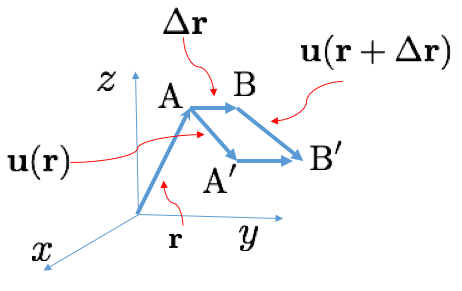
\includegraphics{figures/deform_sketch.png}
 \caption{We use a Cartesian coordinate system. In this system, the
   point A has the position vector $\rr$, and its neighboring point B
 has the position vector $\rr+\Delta \rr$. Under deformation A moves
 to ${\rm A}^{\prime}$ and B moves to ${\rm B}^{\prime}$. The
 deformation at A is $\uu(\rr)$ and the deformation at B is
 $\uu(\rr+\Delta \rr)$. }
  \label{fig:dsketch}
\end{marginfigure}
%
Let us compactify our notation. I use $\ua$ where $\alpha =1,2,3$ for
a component of the vector $\uu$. Let $\rr = (x,y,z)$ and $\Delta\rr =
(\Delta x, \Delta y, \Delta z)$. And I use the symbols 
\begin{subequations}
\begin{align}
a_{11} & =  \duxdx  \/, \quad a_{12} =  \duxdy \/,\quad  a_{13} =
         \duxdz \/, \\
a_{21} & =  \duydx  \/, \quad a_{22} =  \duydy \/,\quad  a_{23} =
         \duydz \/, \\
 a_{31} & =  \duzdx  \/, \quad a_{32} =  \duzdy \/,\quad  a_{33} =
         \duzdz \/,
\end{align} 
\end{subequations}
I can write the equation for deformation to be 
\begin{equation}
\ua(\rr) = \ua(\rr+\Delta \rr) + a_{\alpha\beta} \Delta r_{\beta} + \ldots
\end{equation}
\marginnote{
By $a_{\alpha\beta}\Delta r_{\beta}$ I mean
$\sum_{\beta=1,3}a_{\alpha\beta}\Delta r_{\beta}$. In these lectures
any index, e.g., $\beta$ here, that is repeated is assumed to be
summed -- this is known as the Einstein summation convention.  
}
Remember that the collection of number $a_{\alpha\beta}$ themselves
are function of space, they depend on \textit{where} we calculate the
derivatives.  As long as  $\mid\Delta \rr\mid$ is small enough I can
ignore all the higher order terms that I have denoted by the
triple-dots.  This is assumed in the rest of this discussion. 

\begin{fullwidth}
Now I am going to reorganize the collection of numbers
$a_{\alpha\beta}$ in ``symmetric'' and ``anti-symmetric'' manner: 
\begin{equation}
a_{\alpha\beta} = \frac{a_{\alpha\beta}-a_{\beta\alpha}}{2} +
  \frac{a_{\alpha\beta}+a_{\beta\alpha}}{2}  \/.
\label{eq:break}
\end{equation}
Substituting  back in \Eq{eq:uu} I get
\begin{subequations}
\begin{align}
u_1(\rr+\Delta \rr) &= u_1(\rr) + 
   {\color{red}0 + \frac{a_{12}-a_{21}}{2}\Delta y +
    \frac{a_{13}-a_{31}}{2}\Delta z}  +
       {\color{blue}a_{11}\Delta x+ \frac{a_{12}+a_{21}}{2}\Delta y +
    \frac{a_{13}+a_{31}}{2}\Delta z}\\
u_2(\rr+\Delta \rr) &= u_2(\rr) + 
   {\color{red}\frac{a_{21}-a_{12}}{2}\Delta x + 0 +
    \frac{a_{23}-a_{32}}{2}\Delta z}  +
       {\color{blue}\frac{a_{12}+a_{21}}{2}\Delta x+ a_{22}\Delta y +
    \frac{a_{23}+a_{32}}{2}\Delta z}\\
u_3(\rr+\Delta \rr) &= u_3(\rr) + 
   {\color{red}\frac{a_{31}-a_{13}}{2}\Delta x +
    \frac{a_{32}-a_{23}}{2}\Delta y+ 0}  +
       {\color{blue}\frac{a_{31}+a_{13}}{2}\Delta x+ 
    \frac{a_{23}+a_{32}}{2}\Delta y + a_{33}\Delta z}
\end{align}
\label{eq:u123}
\end{subequations}
\end{fullwidth}
I can now interpret the right-hand-side(RHS) of \Eq{eq:u123} 
as a sum of three displacements, 
\begin{equation}
\uu(\rr+\Delta \rr) = \dd_1+{\color{red}\dd_2}+{\color{blue}\dd_3}
\label{eq:disp}
\end{equation}
The black ones show that two neighboring points are
displaced by exactly the same amount, 
\begin{equation}
\uu(\rr+\Delta \rr) = \uu(\rr) \/,
\end{equation}
this is translation. 

Now organize the red ones
\begin{equation}
{\color{red}\dd_2  = 
\begin{pmatrix}
0 & \frac{a_{12}-a_{21}}{2} &
    \frac{a_{13}-a_{31}}{2}  \\
\frac{a_{21}-a_{12}}{2} &  0 &
    \frac{a_{23}-a_{32}}{2}  \\
\frac{a_{31}-a_{13}}{2} &
    \frac{a_{32}-a_{23}}{2} & 0 
\end{pmatrix}
\begin{pmatrix}
\Delta x \\ \Delta y  \\ \Delta z
\end{pmatrix}
 }
\label{eq:anti}
\end{equation}
The matrix the appears is an anti-symmetric matrix. 
%
 \begin{marginfigure}
  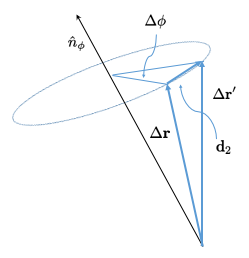
\includegraphics{figures/rotvec.png}
 \caption{Infinitismal rotation by cross-product. Write the vector $\Delta \pphi$
   as a vector pointing in the direction $\hat{n}_{\phi}$ with
   magnitude $\Delta \phi$.  The cross-product of $\Delta \pphi$ and
   $\Delta \rr$ is the vector $\Delta \rr^{\prime}$. }
  \label{fig:rotvec}
\end{marginfigure}

A different but equivalent way to interpreting $\dd_2$ is 
\begin{equation}
\dd_2 = \frac{1}{2}\Delta \pphi \times \Delta \rr
\label{eq:rot}
\end{equation}
where the vector $\Delta \pphi \equiv (\Delta \phi_1,\Delta
\phi_2,\Delta \phi_3)$ is an infinitismal rotation vector
which points along the axis of rotation with a magnitude equal to the 
angle of rotation, with 
\begin{subequations}
\begin{align}
\Delta \phi_1 & =  a_{32}-a_{23} \/, \\
\Delta \phi_2 & =  a_{13}-a_{31} \/,\\
\Delta \phi_3 & =  a_{21}-a_{12} \/.
\end{align}
\end{subequations}
\marginnote{
An infinitismal rotation can be represented by a vector, although
not an ``usual'' vector but a \textit{axial} vector. Rotation by a
finite amount cannot in general be represented by a vector but 
can be represented by an anti-symmetric matrix 
as in \Eq{eq:anti}.
}
Let us now consider the blue terms in \Eq{eq:u123}
\begin{equation}
{\color{blue}\dd_3 = 
\begin{pmatrix}
a_{11} & \frac{a_{12}+a_{21}}{2} &
    \frac{a_{13}+a_{31}}{2}  \\
\frac{a_{21}+a_{12}}{2} &  a_{22} &
    \frac{a_{23}+a_{32}}{2}  \\
\frac{a_{31}+a_{13}}{2} &
    \frac{a_{32}+a_{23}}{2} & a_{33} 
\end{pmatrix}
\begin{pmatrix}
\Delta x \\ \Delta y  \\ \Delta z
\end{pmatrix}
}
\label{eq:sym}
\end{equation}

This is a real symmetric matrix. Hence it can always be diagonalized
by an orthogonal transformation. In other words, by a suitable
rotation of coordinates I can always find a new coordinate system in
which this matrix is diagonal. In that coordinate the displacement $\dd_3$
will have the form
\begin{equation}
{\color{blue}\dd_3 = 
\begin{pmatrix}
\Lambda_{1} & 0 & 0  \\
0 &  \Lambda_{2} & 0  \\
0 & 0 & \Lambda_{3} 
\end{pmatrix}
\begin{pmatrix}
\Delta X_1 \\ \Delta X_2  \\ \Delta X_3
\end{pmatrix}
}
\label{eq:diag}
\end{equation}
You may be already familiar with real symmetric matrices and their properties,
in particular their eigenvalues and eigenvectors from a course on
quantum mechanics where they appear as Hamiltonian or 
from a course in classical mechanics where they appear during the
discussions of moment of inertia of rigid objects. Proofs can be found
in any book on matrices or linear algebra, e.g., Arfken and Weber\cite{Arfken}.

The three $\Lambda$s are the three eigenvalues of the strain matrix
$s_{\alpha\beta}$ given in \Eq{eq:sym}. They must be real, but
they can be either positive or negative. A positive(negative)
$\Lambda$ denotes extension (compression) along the corresponding 
eigenvector $X$. The three eigenvectors are orthogonal to each other,
together they form a Cartesian triad. 
This proves Helmholtz's theorem. 

\section{Strain ellipsoid}
\label{sec:strain_ellipsoid}
One way to visualize the strain matrix is to construct what is called
its ``quadratic form'' , $f(x,y,z) \equiv
r_{\alpha}s_{\alpha\beta}r_{\beta} $
where the vector $\rr = (x,y,z)$ has components $r_{\alpha}$ with
$\alpha=1,2,3$. Written explicitly as
\begin{equation}
f(x,y,z) = 
\begin{pmatrix}
x & y & z 
\end{pmatrix}
\begin{pmatrix}
a_{11} & \frac{a_{12}+a_{21}}{2} &
    \frac{a_{13}+a_{31}}{2}  \\
\frac{a_{21}+a_{12}}{2} &  a_{22} &
    \frac{a_{23}+a_{32}}{2}  \\
\frac{a_{31}+a_{13}}{2} &
    \frac{a_{32}+a_{23}}{2} & a_{33} 
\end{pmatrix}
\begin{pmatrix}
x \\ y \\ z 
\end{pmatrix} 
\label{eq:ellipsoid}
\end{equation}
The function $f(x,y,z)$ is in general a quadratic in all its
arguments. Setting it equal to unity (or any other constant) defines a
surface in three dimensional space. This surface is called a {\textit strain
ellipsoid}. Geometrically, it is an actual ellipsoid only if all the
three eigenvalues of the strain matrix are positive.
% 
 \begin{marginfigure}
  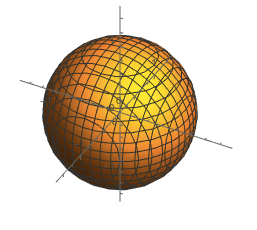
\includegraphics[width=0.8\textwidth]{figures/qsurf1.png}
  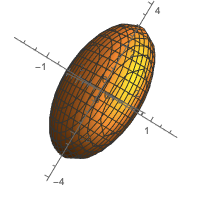
\includegraphics[width=0.8\textwidth]{figures/qsurf2.png}
  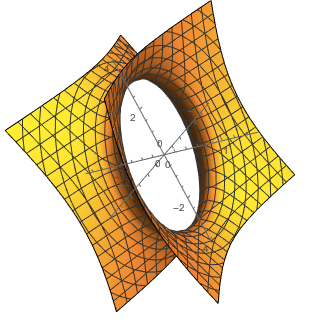
\includegraphics[width=0.8\textwidth]{figures/qsurf3.png}
 \caption{ Visualization of quadratic surfaces in three
   dimensions. The top one is a sphere with the equation
  $x^2+y^2+z^2=1$. The middle one is an ellipsoid 
  $4x^2+\frac{y^2}{4}+\frac{z^2}{9}=1$. The bottom one is
 $-4x^2+\frac{y^2}{4}+\frac{z^2}{9}=1$. These are the equations of
 these surfaces in terms of their eigencoordinates which are the axes
 shown in the figure. }
  \label{fig:qsurf}
\end{marginfigure}
%
A complete classification of quadratic surfaces can be found at 
\url{http://mathworld.wolfram.com/QuadraticSurface.html}. You should
use a visualization software  to play with quadratic
surface. The three simplest examples given in the margin are plotted
using Mathematica.
\section{Vorticity}
Let us now pass from displacement to velocity. We write the total
displacement $\uu$  as $\uu = \vv \Delta t$ and the infinitismal
rotation vector as $\Delta \pphi = \oo \Delta t$. In terms of
components this becomes 
\begin{subequations}
\begin{align}
u_1 = v_1 \Delta t \quad u_2 = v_2 \Delta t \quad u_3 = v_3 \Delta t
  \\
\Delta \phi_1 = \omega_1 \Delta t \quad \Delta \phi_2 =
  \omega_2 \Delta t\quad
  \Delta \phi_3 = \omega_3 \Delta t 
\end{align}
\end{subequations}
The vector $\oo$ is called the vorticity vector. You should
explicitly check that $\oo$ and  $\vv$ are related by  
\begin{equation}
\oo = \curl \vv
\end{equation}
The vorticity vector plays a crucial role in understanding the
behavior of fluids. 
\begin{Exercise}
\Question
To reinforce the idea that the displacement $\dd_2$ is indeed a
rotation show that under this displacement the length of the vector
$\Delta \rr$ remains unchanged. In particular, show that the two
vector $\Delta r$ and $\Delta r^{\prime}$ have the same length. 
\Question Consider the quadratic form in two variables
\begin{equation}
2x^2 + 5xy+ 3y^2 = 1
\end{equation}
Write this in a form similar to the RHS of \Eq{eq:ellipsoid}, you
should get a $2\times 2$ matrix. Diagonalize this matrix, find its
eigenvalues and eigenvectors. Sketch the two eigenvectors in the $x-y$
coordinate system. 
\end{Exercise}
\begin{subappendices}
\section{Who is afraid of Cartesian Tensors?}
I have so far interpreted the strain as a $3\times 3$ matrix at every
point in space. It is also viewed as a second rank tensor field. 
Any old collection of nine numbers at every point in space does not
make a tensor field, just like any collection of three numbers does
not make a vector field. They must satisfy the correct
\textit{transformation laws}. 
\marginnote{Here, by coordinate transformation I mean only rotation of
  coordinates. The transformation properties under
  more general, nonlinear coordinate transformation gives rise to more
  general non-Cartesian tensors -- they become useful while studying
  the general theory of relativity.}
 A scalar field, which a single number
at every point is space must be invariant under coordinate
transformation. Any vector quantity does not remain invariant, but must change
exactly like (remain \textit{covariant})  distance between two points
under coordinate transformation. A vector is a tensor of rank one, the
strain is a tensor of rank two. The vorticity can be either thought of
as a tensor of rank one, i.e., a vector but it is a \textit{polar}
vector, one that changes sign under the coordinate transformation
$x\to -x$, $y\to -y$ and $z\to -z$. Or it can be interpreted as a
second rank anti-symmetric tensor. In this course I assume you know
what a vector is, but not what a second or higher rank tensor is --
second or higher rank tensor are common occurrence in fluid mechanics,
I enthusiastically recommend a wonderful book by Rutherford
Aris~\cite{Aris} for a comprehensive introduction to this subject. 
During this course we shall learn tensors as and when we need them,
starting now. 

Consider a coordinate system $\{x_1,x_2,x_3\}$. We do a linear
transformation and obtain a new coordinate system
$\{y_1,y_2,y_3\}$. The linear transformation that relates them is give
by 
\begin{equation}
y_{\alpha} = a_{\alpha\beta} x_{\beta}\/,
\label{eq:transform}
\end{equation}
where $\alpha,\beta$ runs from $1$ to $3$ and we have again assumed
 the Einstein summation convention. A typical example is rotation about
 an axis, as shown in \Eq{eq:2drot}. 
\marginnote{
 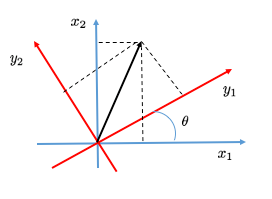
\includegraphics{figures/2drot.png} \\
An example of linear transformation of coordinates. The two
   Cartesian coordinate systems are related to each other by a
   rotation by the angle $\theta$ along an axis perpendicular to the
   plane. The same point in space are now labeled by two different
   coordinate systems $(x_1,x_2)$, and $(y_1,y_2)$ related to each
   other by 
\begin{equation}
\begin{pmatrix}
y_1 \\ y_2
\end{pmatrix}
=
\begin{pmatrix}
\cos\theta & -\sin\theta \\
\sin\theta & \cos\theta 
\end{pmatrix} 
\begin{pmatrix}
x_1 \\ x_2
\end{pmatrix}
\label{eq:2drot}
\end{equation}
 }
The magnitude of the position vector remains unchanged under rotation;
hence
\begin{equation}
y_{\alpha}y_{\alpha} = a_{\alpha\beta}a_{\alpha\mu} x_{\beta}x_{\mu}
= x_{\mu}x_{\mu} \/.
\end{equation}
Then we must have 
\begin{equation}
a_{\alpha\beta}a_{\alpha\mu} = \delta_{\beta\mu}
\label{eq:delta}
\end{equation}
where $\delta_{\beta\mu}$
\begin{equation}
\delta_{\beta\mu} =
\begin{cases} 1 \/, & \quad\quad {\rm for} \beta = \mu \\
  0 \/,& \quad\quad {\rm otherwise}
\end{cases}
\end{equation}
is called the ``Kronecker delta''. You also know it as the identity matrix
\begin{equation}
\mathbb{1} = 
\begin{pmatrix}
1 & 0 \\
0 & 1
\end{pmatrix}
\end{equation}
Let us check \Eq{eq:delta} explicitly with the matrix $a_{\alpha\beta}$
given in \Eq{eq:2drot}:
\begin{subequations}
\begin{align}
\beta=1\/,\mu=1&\/ \quad\quad a_{11}a_{11} + a_{21}a_{21} =
  \cos^2\theta+\sin^2\theta = 1 \\
\beta=1\/,\mu=2&\/ \quad\quad a_{11}a_{12} + a_{21}a_{2} =
  \cos\theta\sin\theta-\cos\theta\sin\theta = 0 
\end{align}
\end{subequations}
\marginnote{ Multiply both sides of \Eq{eq:Ap} by $a_{\sigma\alpha}$ and sum over
the repeated index $\alpha$ to get
\begin{eqnarray}
a_{\alpha\sigma}\Ap_{\alpha} &=
  a_{\alpha\beta}a_{\alpha\sigma}A_{\beta}  \nonumber \\
\implies a_{\alpha\sigma}\Ap_{\alpha}&= \delta_{\beta\sigma}A_{\beta}
  = A_{\sigma} \nonumber \\
\implies A_{\alpha} &= a_{\beta\alpha}\Ap_{\beta} \/. \nonumber
\end{eqnarray}
In the second line above we have use \Eq{eq:delta}.
}
A vector is defined to be a quantity that transforms just like the
position vector under the same coordinate transformation, i.e., if any
vector $\AA= (A_1,A_2,A_3)$ in the coordinate system $(x_1,x_2,x_3)$
transforms to $\AAp = (\Ap_1,\Ap_2,\Ap_3)$ under the coordinate
transformation given in \Eq{eq:transform} then 
\begin{equation}
\Ap_{\alpha} = a_{\alpha\beta} A_{\beta}
\label{eq:Ap}
\end{equation}
We can invert \Eq{eq:Ap} to obtain
\begin{equation} 
 A_{\alpha} = a_{\beta\alpha}\Ap_{\beta} \/.
\label{eq:invert}
\end{equation}
In other words, the inverse of the matrix $a_{\alpha\beta}$ is its
transpose. This is a property of the rotation matrix that you may
already know. This is a consequence of demanding that the length of
vectors remain unchanged under the transformation \Eq{eq:transform}. 

Now let us try to find out how $s_{\alpha\beta}$ transforms
under the same coordinate transformation. Start with \Eq{eq:sym}
which we now write in compact notation as 
\begin{equation}
d_{\alpha} = s_{\alpha\beta}r_{\beta}
\end{equation}
Here for notational simplicity we have used $\rr$ instead of the
symbol $\Delta \rr$. 
As $\dd$ is a vector, its transform $\dd^{\prime}$ will satisfy an 
equation like \Eq{eq:invert}. Hence
\begin{equation}
a_{\mu\alpha}d^{\prime}_{\mu} = s_{\alpha\beta}r_{\beta}
\end{equation} 
Multiplying both sides by $a_{\kappa\alpha}$ and summing over the
repeated index $\alpha$ and subsequent simplification we obtain
\begin{equation}
d^{\prime}_{\kappa} =
  a_{\kappa\alpha}a_{\gamma\beta}s_{\alpha\beta}r^{\prime}_{\gamma}
\label{eq:ss}
\end{equation}
\marginnote{
The intermediate steps works out in the following manner:
\begin{eqnarray}
d_{\alpha} &= s_{\alpha\beta}r_{\beta} \nonumber \\
\implies a_{\mu\alpha}d^{\prime}_{\mu} &= s_{\alpha\beta}r_{\beta}
  \nonumber \\
\implies a_{\kappa\alpha}a_{\mu\alpha}d^{\prime}_{\mu} &=
  a_{\kappa\alpha}s_{\alpha\beta}r_{\beta} \nonumber \\
\implies \delta_{\kappa\mu}d^{\prime}_{\mu} &=
  a_{\kappa\alpha}s_{\alpha\beta}r_{\beta} \nonumber \\
\implies d^{\prime}_{\kappa} &=
  a_{\kappa\alpha}s_{\alpha\beta}r_{\beta} \nonumber \\
\implies d^{\prime}_{\kappa} &=
  a_{\kappa\alpha}a_{\gamma\beta}s_{\alpha\beta}r^{\prime}_{\gamma}
\nonumber
\end{eqnarray}
}
In the transformed (primed) coordinate system we should have 
\begin{equation}
d^{\prime}_{\kappa} = s^{\prime}_{\kappa\gamma}r^{\prime}_{\gamma}
\label{eq:sprime}
\end{equation}
Comparing \Eq{eq:ss} and \Eq{eq:sprime} we obtain the transformation
law for the strain
\begin{equation}
\boxed{s^{\prime}_{\kappa\gamma} = a_{\kappa\alpha}a_{\gamma\beta}s_{\alpha\beta}}
\end{equation}
We have now proved that the strain is a second rank tensor. In
general, any linear relationship between two vectors of the form
\begin{equation}
A_{\mu} = T_{\mu\nu}B_{\nu}
\label{eq:quotient}
\end{equation}
implies that the quantity $T_{\mu\nu}$ is a second rank tensor. 
This is sometimes called the ``quotient rule''. 
This is a very useful way to find out what kind of tensor a physical
quantity is. Two other examples where this rule is used are the moment of inertia tensor, or the polarizability
tensor of a medium. 

\subsection{Fully anti-symmetric tensor}
Let us revisit the displacement $\dd_2$
\begin{equation}
\dd_2  = 
\begin{pmatrix}
0 & \frac{a_{12}-a_{21}}{2} &
    \frac{a_{13}-a_{31}}{2}  \\
\frac{a_{21}-a_{12}}{2} &  0 &
    \frac{a_{23}-a_{32}}{2}  \\
\frac{a_{31}-a_{13}}{2} &
    \frac{a_{32}-a_{23}}{2} & 0 
\end{pmatrix}
\begin{pmatrix}
\Delta x \\ \Delta y  \\ \Delta z
\end{pmatrix}
\label{eq:anti2}
\end{equation}
where $a_{\alpha\beta} = \partial_{\beta} u_{\alpha}$.
In \Eq{eq:rot} we interpreted this equation as 
\begin{equation}
\dd_2 = (1/2) \Delta \pphi \times \Delta \rr 
\end{equation}
 To make a clearer connection to
vorticity let us write
\begin{equation}
\dd_2 = (1/2) \oo \times \Delta \rr \Delta t 
\end{equation} 
where 
\begin{equation}
\omega_1 = \partial_2v_3 - \partial_3v_2 \quad 
\omega_2= \partial_3v_1 - \partial_1 v_3 \quad 
\omega_3 = \partial_1v_2 - \partial_2 v_1 
\end{equation}
\marginnote{
I shall use either $\{x,y,z\}$ or $\{x_1,x_2,x_3\}$ or $\{x_{\mu}\}$ to denote
Cartesian coordinate systems.
I shall use bold fonts for vector, e.g., $\AA$, $\Delta \bm{r}$
etc. I shall write the individual components of the vector $\AA$ as
either $A_x,A_y,A_z$, or $A_1,A_2,A_3$ or collectively $A_{\mu}$. I
shall typically use Greek indices to denote components of vectors or
tensors. The convention can be extended in a straightforward way to
denote any component of a higher rank tensor, e.g., $T_{\alpha\beta}$
. Sometime I shall use the same symbol to denote the higher rank
tensor itself. The symbols $\frac{\partial}{\partial x}$,
$\partial_x$, $\partial_1$ will all mean the same thing, with the
symbol $\partial_{\mu}$ denoting partial derivative with respect to a
general coordinate $x_{\mu}$. 
}
Clearly,  \Eq{eq:anti2} can also be written as 
\begin{equation}
(d_2)_{\alpha} = (1/2)\Omega_{\alpha\beta} \Delta r_{\beta} \Delta t
\end{equation}
where  
\begin{equation}
\Omega_{\alpha\beta} = 
\begin{pmatrix}
0 & -\omega_3  & \omega_2 \\
\omega_3 & 0 & -\omega_1 \\
-\omega_2  & \omega_1 & 0 
\end{pmatrix}
\end{equation}
By the quotient rule the set of number $\Omega_{\alpha\beta}$ 
constitutes a second rank tensor, that is anti-symmetric. 
The vector $\oo$ and the second rank tensor $\Omega_{\alpha\beta}$ 
can be related to each other by, you guessed it, a \textit{third} rank
tensor :
\begin{equation}
\Omega_{\alpha\beta} = \epsilon_{\alpha\beta\gamma}\omega_{\gamma}
\end{equation}
This is called  the Levi-Civita tensor
\begin{equation}
\epsilon_{\alpha\beta\gamma} =
\begin{cases}
 0 \/,&\quad \text{ if any two of them are equal.} \\
1 \/,&\quad \text{ for even permutation} \\
-1 \/,& \quad \text{ for odd permutation}   
\end{cases} 
\end{equation}
\marginnote{
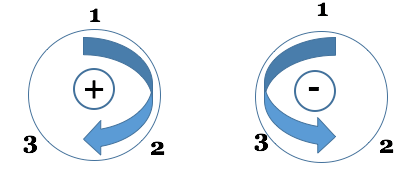
\includegraphics{figures/cross.png} \\
The only non-zero elements of $\epsilon_{\alpha\beta\gamma}$ are
\begin{eqnarray}
\epsilon_{123} &= \epsilon_{231}=\epsilon_{312} =1 
\nonumber \\
\epsilon_{132} &= \epsilon_{321}=\epsilon_{213} =-1 
\nonumber 
\end{eqnarray}
}
Using the  Levi-Civita tensor the cross-product of two vectors can be
written as
\begin{equation}
(\AA\times\BB)_{\alpha} = \epsilon_{\alpha\beta\gamma}A_{\beta}B_{\gamma}
\end{equation}
\end{subappendices}


%----------------------------------------------------------------------------------------
%	CHAPTER 2
%----------------------------------------------------------------------------------------
\chapter{Hydrostatics}
\label{ch:hydrostatics}
\section{Stress}
Let us now get back to the piece of ``slime'' we started the last
lecture with. Consider a small volume element inside the slime. There
are forces acting of this small volume element due to the rest of the
slime. These forces act through the surface of the volume element.
Let us be specific and consider a small box (a rectangular
parallelepiped) of slime with its center at $x,y,z$, lying between 
$x-(1/2)\Delta x $ to $x+(1/2)\Delta x$, 
$y-(1/2)\Delta y$ to $y+(1/2)\Delta y$, and 
$z-(1/2)\Delta z$ to $z+(1/2)\Delta z$.
Consider the face at $x+(1/2)\Delta x$. There is a force by the rest of the
slime acting through this face. Let us call this force
$\ff(x+(1/2)\Delta x,y,z)$. In general, this force can point in
any direction, i.e., it can have all the three components,
$f_x(x+(1/2)\Delta x,y,z)$, $f_y(x+(1/2)\Delta x,y,z)$ and 
$f_z(x+(1/2)\Delta x,y,z)$. The force not only depends on space
(i.e., $x,y,z$) but also which face we are considering. At the same
point $x+(1/2)\Delta x,y,z$ we can consider two different planes,
one perpendicular to the $x$ axis, given by $\Delta y \times \Delta
z$, and another perpendicular to the $z$ axis, given by $\Delta y
\times \Delta x$. The force $\ff$ on these two infinitismal area
elements are clearly different. To emphasize that we label each
component of the force accordingly. Each area element can be uniquely labeled by
the direction of the unit vector normal to it. So the force components
of the force acting at $(x+(1/2)\Delta x,y,z$ on the face of the
cube perpendicular to the $x$ direction is labeled by
$xx$, $xy$ and $xz$. 
\begin{marginfigure}
  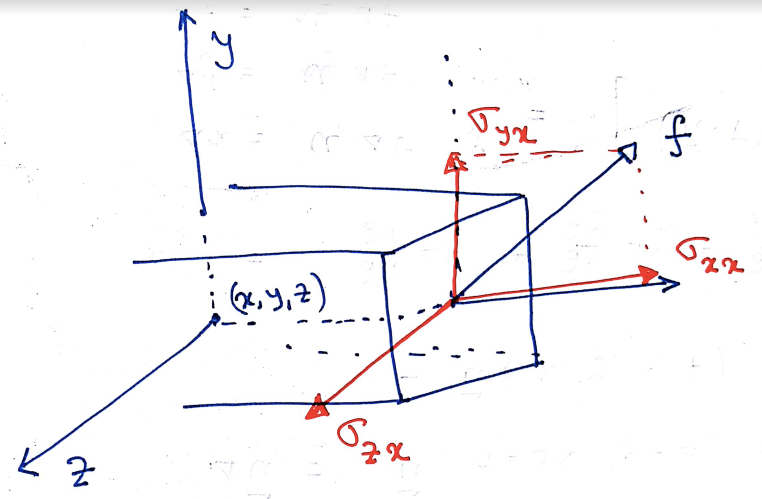
\includegraphics{figures/stress.png}
 \caption{ The force on the face $\Delta y\Delta z$ due to the rest of
 the material is $\ff$. It has components along the three axis,
 $\sigma{xx}$, $\sigma_{yx}$, $\sigma_{zx}$.  If you consider a 
different face at the same point, e.g., $\Delta x\Delta y$, 
the force will be different.}
  \label{fig:stress}
\end{marginfigure}
 Next we define, the force per-unit-area as:
\begin{subequations}
\begin{align} 
\sigma_{xx}(x+(1/2)\Delta x,y,z) \Delta y\Delta z&= f_x(x+(1/2)\Delta x,y,z)\/, \\
\sigma_{yx}(x+(1/2)\Delta x,y,z) \Delta y \Delta z&= f_y(x+(1/2)\Delta x,y,z)\/,
{\rm  and} \\ 
\sigma_{zx}(x+(1/2)\Delta x,y,z) \Delta y \Delta z  &= f_z(x+(1/2)\Delta x,y,z)\/. \end{align}
\end{subequations}
Similarly we can define a set of nine number $\sigma_{\alpha\beta}$.
More compactly, the force acting on an area element $\Delta S$ with
its unit normal $\nhat$ is given by 
\begin{equation}
f_{\alpha} = \sigma_{\alpha\beta}n_{\beta}\Delta S \/.
\end{equation}
As $\ff$ is a vector, by the quotient rule $\sigma_{\alpha\beta}$ is 
a second rank tensor.  This is called the ``stress tensor''.

\begin{fullwidth}
Let us try to calculate the total
force on the volume element $\Delta x\Delta y\Delta z$. 
We have to sum over each component of the
force through all the faces. Let us first sum the  $y$ component along
the two faces perpendicular to the $x$ axis:
\begin{subequations}
\begin{align}
f_y(x+\frac{1}{2}\Delta x,y,z)&+f_y(x-\frac{1}{2}\Delta x,y,z) 
= \left[ \sigma_{yx}(x+(1/2)\Delta x,y,z)-  \sigma_{yx}(x-(1/2)\Delta
  x,y,z) \right] \Delta y\Delta z \nonumber \\
&=\left[ \{\sigma_{yx}(x,y,z) + \partial_x \sigma_{yx}\mid_{x,y,z}\frac{\Delta x}{2} +\ldots\}
            -  \{\sigma_{yx}(x,y,z) - \partial_x
  \sigma_{yx}\mid_{x,y,z}\frac{\Delta x}{2}+ \ldots\}  \right]\Delta y \Delta z
  \nonumber \\
&= \partial_x \sigma_{yx} \Delta x\Delta y\Delta z + \ldots \nonumber \\
\end{align}
\end{subequations} 
\end{fullwidth}
Here we have expanded $\sigma_{yx}$ in a Taylor series and truncated
at the leading order term.  Doing this for all the components over all
the faces, we get the total force $\FF$ on the volume element 
$\Delta V = \Delta x\Delta y\Delta z$ as 
\begin{equation}
F_{\beta} = \partial_{\alpha}\sigma_{\beta\alpha}\Delta V 
\label{eq:divs}
\end{equation}
%
 \begin{marginfigure}
  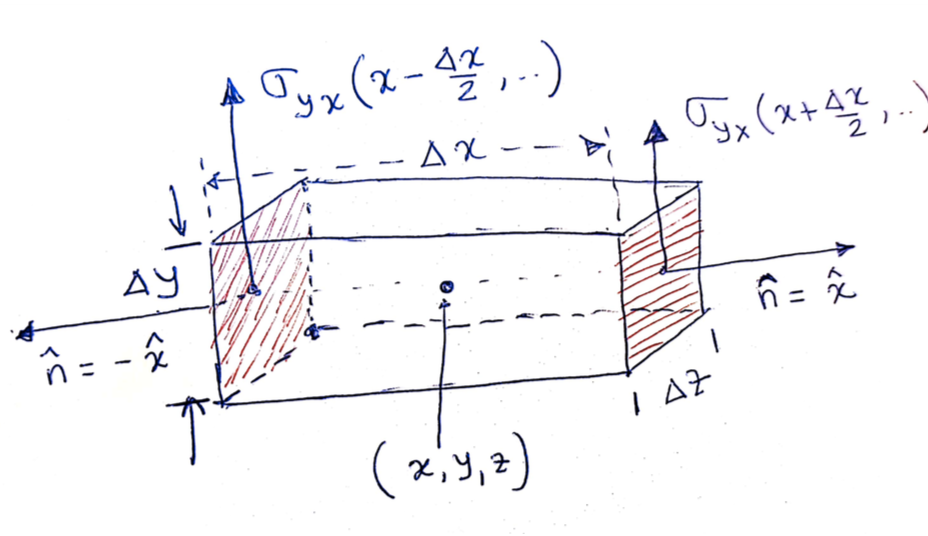
\includegraphics{figures/DivStress.png}
 \caption{ The force on the volume $\Delta x\Delta y\Delta z$ along
   the $y$ direction due to the forces on the two faces that are at
   $x-\Delta x$ and $x+\Delta x$. The force on each face comes from the
   $\sigma_{yx}$  component of the stress multiplied by the 
   area-element  $\nhat\Delta y\Delta z$. The unit vector $\nhat =
   \xhat$ for the face at $x+\Delta x$ and $\nhat=-\xhat$ for the face
 $x-\Delta x$. }
  \label{fig:DivStress}
\end{marginfigure}
%
Here $\FF$ is a vector and $\sigma_{\alpha\beta}$ is a second rank
tensor, then by the quotient rule the components of the operator
$\partial_{\alpha}$ forms a vector, this is the usual gradient
operator 
\begin{equation}
{\bm \nabla} = (\xhat\frac{\partial}{\partial x}+\yhat\frac{\partial}{\partial y}+\zhat\frac{\partial}{\partial z} ) 
\end{equation}
Thus you may think of RHS of \Eq{eq:divs} as the divergence of the
stress tensor. You need to be careful about one point though, although
the RHS of \Eq{eq:divs} is often called a divergence it is not a
scalar as usual divergence of a vector field is, but a vector; thus it
is not invariant under rotation. 

By Newton's laws the force $\FF$ is mass times acceleration of the
small volume element $\Delta V$. Let us now associate a density and a
velocity to every point of a deformable body, $\rho(x,y,z)$ and 
$\vv(x,y,z)$.  The equation of motion then becomes
\begin{equation}
\boxed{
\rho\frac{dv_{\alpha}}{dt} = \partial_{\beta}\sigma_{\alpha\beta}
}
\end{equation}

\section{What is a fluid ?}

As the subject of these lectures is \textit{fluid} mechanics I have been
guilty of not even defining what a fluid is. So far I have talked about
kinematics of deformable objects, whatever I have said applies to both
deformable solid -- all solids are deformable -- and fluids. From the
point of view of continuum mechanics -- the view that we adopt in
these lectures -- a fluid is such a material in which at a steady
state the off-diagonal components of the stress tensor must be
zero. This may seem to be a very abstract definition of a fluid, so
let me try to state it more simply. The diagonal components of stress
tensor is  either compressive or extensional. They can either dilate or
compress a material. But an off-diagonal component is a shear.
So the ``definition'' of fluid can be stated simply as: `` under shear,
fluid flows''. Interpreted differently, this is also the simplest
definition of a fluid: `` a fluid at rest always takes the shape of
its container''.  Clearly most materials we consider as fluid, e.g.,  air,
water, wine, oil satisfies this definition. But what about mud or
cement ? It depends on how ``thick'' the mud is and also \textit{ how
  long} you wait till you for it to reach a steady state. Given enough
time -- geological time-scales -- even mountains flow. 
So this definition of fluid depends on the time-scale over which you ask
the question.  Alternatively, we can try to define fluid by its
structure: it is easier to define a solid first. The molecules in a
solid are organized on a regular lattice. By contrast, in a fluid they
are not. But there is something else the behaves like a solid as far
las stresses are concerned but its structure is close to liquids than
to solids : glasses.  Maybe glasses are actually liquids that flows
very very slowly ? Glass windows in old cathedrals are often found to
be uneven, typically thicker at the bottom. But estimates show that 
these are not evidences of flow of glass: `` window glasses may flow 
at ambient temperature only over incredibly long times, 
which exceed the limits of human
history.''\cite{zanotto1998cathedral,zanotto1999cathedral}. 
At the moment, the consensus among scientists is that glass are a
new phase of matter, neither liquids nor solids, but this is still
very much an active field of research. 
To summarize, in the rest of these lectures I shall use the definition of fluid I gave at the
beginning of this section, but be aware that the definition has
nuances. 

\section{Fluid at rest}
By the definition of the fluid at rest, the stress tensor can not have
any off-diagonal component, it must have only diagonal components.
Hence for a fluid 
\begin{equation}
\sigma_{\alpha\beta} = 0 \quad\text{for $\alpha\neq\beta$} 
\label{eq:statics}
\end{equation}
The tensor quadratic of this tensor is then an ellipsoid. 
But the expression in \Eq{eq:statics} is a physical law, hence must be true in all
coordinate systems, the tensor quadratic must then be a sphere
the only ellipsoid that is invariant under rotation of coordinate
systems. The stress at every point in a fluid at rest can then be
specified by just a single number, 
\begin{equation}
\sigma_{\alpha\beta} = -p \delta_{\alpha\beta}\/,
\label{eq:pressure}
\end{equation}
the pressure, a scalar. Note the sign in \Eq{eq:pressure}. 
Strictly speaking the the stress can be both positive or negative and
in a solid it can have both signs, but in a liquid the stress is
always a compression. We have emphasized this with the negative sign
in \Eq{eq:pressure}. Blaise Pascal, as far as I know, was the first to perceive
this law. 

Notice that so far we have not considered any external forces, e.g,
gravity.  If the force can be obtained as the negative gradient of a potential
$\Phi$, the state of mechanical equilibrium of a fluid
at rest is then given by 
\begin{equation}
-\grad p - \grad \Phi = 0 
\label{eq:fstatics}
\end{equation}
\marginnote{
\begin{equation}
\partial_{\alpha}\sigma_{\beta\alpha}
= -\partial_{\alpha}p\delta_{\beta\alpha} = -\grad p \nonumber
\end{equation}
}
This equation can be integrated\footnote{But watch out for what is
  going to come later in section~\ref{sec:multi}.} to obtain 
\begin{equation}
p + \Phi = {\rm constant}
\label{eq:pot}
\end{equation}
The constant must be determined from normalization of the potential
and pressure. 

In principle, the story of hydrostatics is now over.  Let us work out
a few illustrative examples.
\subsection{Units, numerical values}
The unit of pressure (or stress in general) is force-per-unit-area,
which in SI units is ${\rm Newton}{\rm meter}^{-2}$ defined to be one
Pascal. The standard atmospheric pressure is $76 {\rm cm}$ mercury.
Consider a column of mercury of height $h = 76 \cm$ and cross-section
$\Delta A$. The gravitational force at the base is $F= h \rho_{\rm
  mercury} g \Delta A$ and the pressure is 
which is 
\begin{eqnarray}
p_{\rm atm} =&\frac{F}{\Delta A} = h\rho_{\rm mercury} g =
76 \times 10^{-2} \meter \times 13.596 \frac{\gram}{\cm^3} \times 10 \frac{\meter}{\sec^2} \nonumber
\nonumber   \\
=&76 \meter\times 10^{-2} \times 13.596 \times \frac{10^{-3}\kg}{10^{-6}
  \meter^3} \times 10 \frac{\meter}{\sec^2} \nonumber \\
=&76\times 13.596\times 10^{2} \frac{\meter^2\kg  }{\meter^3\sec^2}
    \approx 103 {\rm kPa}  \nonumber
\end{eqnarray}
where ${\rm Pa} =  \kg\meter^{-1}\sec^{-2}$. This demonstrates how
small one Pascal is.  The standard atmospheric pressure is about
hundred kilo Pascal ! 
\subsection{Isothermal atmosphere}
Often the external potential comes from gravity, 
\begin{equation}
\Phi = \rho\Psi
\end{equation}
where $\Psi$ is the gravitational potential. 
The simplest problem in this genre is an ideal gas under isothermal
conditions. In the case the ideal gas law tells us $pV = N\kB T$
where $N$ is the total number of molecules in a volume $V$, with
temperature $T$ and the Boltzmann constant $\kB$. This implies,
$p=n\kB T $ where $n=N/V$ is the number of molecules-per-unit-volume. 
Let us assume that the gas is made out of a single type of gas
molecule each of which has mass $m$. Then 
$p=\rho\kB T/m $. Equation~\ref{eq:fstatics} then takes the form
\begin{subequations}
\begin{align}
\left(\frac{\kB T}{m}\right)\frac{d}{dz} \rho &= -\rho g  \\
\implies \rho(z) &= \rho(z=0)\exp(-\frac{mgz}{\kB T})
\end{align}
\end{subequations}
The assumption of isothermal atmosphere is not very accurate for our
planet; the actual behavior seen in the atmosphere is somewhat
different as discussed by Falkovich~\cite{Falkovich2018fluid}.
%\subsection{Stability of a boat}
\marginnote{ There are two issues with this Problem~\ref{prb2.1}. First, in the laboratory
  frame of reference this problem is really a problem of dynamics not
  of statics, so this does not belong here. This is true for all
  problems that involve centrifugal forces. Secondly, there is no
  {\textit a priori} reason to think that if you do the experiment you
  shall find the a steady solution even in the frame of the rotating
  bucket. The solution we find may simply be an unstable solution and
  some other physical behavior may be realized. } 
\begin{Exercise}
\Question
\label{prb2.1}
{\bf A bucket rotating about its own axis.}\\
Let us consider a bucket rotating about its own axis -- a
centrifuge. In the frame of the bucket the flow is at rest. What is
the shape of (the surface of) water in the bucket ? \\
Let us use cylindrical coordinate system with the $z$ axis of the
cylindrical coordinate system coinciding with the axis of rotation. 
If the bucket is rotating with an angular velocity $\Omega$, the
centrifugal force, on a volume element of size $\Delta V$ at a 
point ($r,\phi,z$) points in radially outward direction, 
$\FF = \rhat F_{r} = \rhat \rho\Delta V \Omega^2r$. The corresponding
potential is defined to be 
$-\frac{\partial\Phi(r)_{\rm cfg}}{\partial r} =   \rho\Omega^2r$.
The total potential is given by $\Phi(r)_{\rm cfg}$ and the potential
due to gravity, $\Phi_{\rm g}(z)$. The potential appearing in  
 \Eq{eq:pot} is the sum of these two potentials.  This gives the
 pressure as a function of $r$ and $z$ including an arbitrary
 constant. The pressure that appears here is the pressure over and
 above the atmospheric pressure which we assume is zero. The equation
 for the free surface is then given by $p(r,z) = 0$. Show that this
 surface is a paraboloid of revolution. 

%\begin{marginfigure}
 % 
\includegraphics{figures/shape_of_water.png}
%\caption{}
%\end{marginfigure}
% 
\Question
{\bf Stress in your bones.} \\
Model your body to be supported two cylindrical pillars which are your
legs. What is the pressure on them at their base ? Now think about a
giant who is $12$ times bigger than you in all directions -- that is
how Gulliver described the Brobdingnags. Estimate the stress suffered
by the bones of those giants. The stress that can break human bones is
estimated to be about $170 {\rm M Pa}$. Can the Brobdingnags have
bones made out of the same material as ours ? What is the stress in
your bones when you jump down from a height of $1\meter$ ?  
\end{Exercise}
\subsection{A multi-valued potential ?}
\label{sec:multi}
I found the following discussion in on page 47-48 in the book by
Sommerfeld\cite{SomII06}. This is so fascinating that I am
going to reproduce this almost verbatim. 

Sommerfeld comments that while integrating \Eq{eq:fstatics}
to obtain \Eq{eq:pot} it is necessary but not sufficient that the potential $\Phi$
exists, it must also be {\textit single-valued}. He illustrates this
comment by discussing one specific, ingenious problem where the potential is not
single-valued. 

Consider a weakly conducting fluid such as a solution
of copper-sulphate placed in a shallow cylindrical container with
insulating bottom and conducting side walls. A copper wire runs along
the axis of the container. A potential difference of a few volts is
put between the center wire and the side wall so as to maintain a
current flowing from the axis through the fluid and spreading out
towards the wall.
We use a cylindrical coordinate system, $r,\phi,z$ with the $z$ axis
pointing along the axis of the container. 
 Let $I$ be the current and $\JJ$ the vector of
current density, $\mid \JJ \mid$ being the current passing radially
through the unit of area at the distance $r$ from the axis. Obviously
\begin{equation}
\mid \JJ(r) \mid = \frac{I}{2\pi r h}\quad,
\end{equation}
\begin{marginfigure}
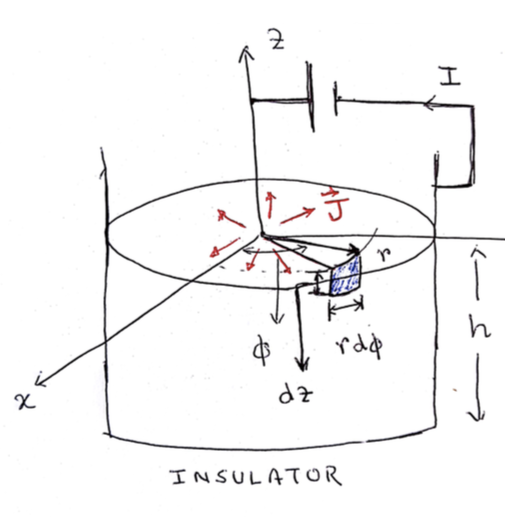
\includegraphics{figures/SomExp.png}
\caption{A sketch of the experiment suggested by Sommerfeld. }
\end{marginfigure}
where $h$ is the height of the fluid layer. 
We now impose a fairly homogeneous magnetic field $\HH$ 
pointing along the axis of the cylinder. The electromagnetic force
acting upon a fluid element of unit volume is given by 
\begin{equation}
\FF = \JJ \times \HH 
\end{equation}
pointing along the azimuthal direction $\ep$, 
\begin{equation}
\FF = \ep F_{\phi} = \frac{A}{r} \quad\text{where}\quad A = \frac{I
  H}{2\pi h} 
\end{equation}
This force has a potential given by 
\begin{equation}
\Phi = - A \phi \/,
\end{equation}
as can be explicitly checked by taking the negative gradient of $\Phi$
to obtain $\FF$. Remarkably this potential is not single valued, as
$\phi$ is a multiple valued function, it changes its value by $2\pi A$
for each revolution of the variable $\phi$ about the $z$-axis. 
But hydrostatic pressure must be a single valued function of
position. Hence \Eq{eq:pot} cannot be satisfied. This implies that in
this case there is no {\textit hydrostatic} solution to the problem,
the setup will give rise to a flow along the azimuthal direction. 
\section{Stability of hydrostatic solution}
There is one last point to remember. Although it is fairly easy to
obtain a hydrostatics solution it need not always be the solution. For
example consider a pot of water on a stove. Put a few tea leaves in
the water such that you can see what whether the water has a motion or
not. If the heating is very low you shall find all the tea leaves at
the bottom of the pot, but if you touch the top of the surface of the
water you shall find it warm. Heat is being transported through water
but by {\textit conduction}, in the way it is transported through a
solid material. This is a situation in hydrostatics. But if the
heating at the bottom in larger than a threshold, the tea leaves are
set into motion. For a even larger heating you can see bubbles rising
and water boiling. The hydrostatic solution has become {\textit
  unstable} and given rise to motion. This is not the place to go into
the stability problem, we shall spend several lectures on them at a
later stage. 
%----------------------------------------------------------------------------------------
\newpage
\section*{Summary of Act 1}
\begin{thm-non}
The most general motion of a sufficiently small element of a
deformable (i.e., not rigid) body can be represented as the sum of 
\begin{enumerate}
\item a translation
\item a rotation
\item an extension (contraction) in three mutually orthogonal
  directions. 
\end{enumerate}
\end{thm-non}
This is a consequence of a general theorem about tensors:
\begin{thm-non}
Any second rank tensor can be decomposed into one
anti-symmetric and one symmetric tensor.  Any anti-symmetric second
rank tensor can be presented as an (axial) vector. 
\end{thm-non}
The motion of a deformable body, solid or liquid, is given by 
\begin{equation}
\rho\frac{dv_{\alpha}}{dt} = \partial_{\beta}\sigma_{\alpha\beta}
\nonumber
\end{equation}
where $\rho$ is the density, $\vv$ is the velocity with components
$v_{\alpha}$,
and $\sigma_{\alpha\beta}$ is the stress tensor at a point $\rr$. 
\begin{def-non}
The off-diagonal components of the shear stress in a fluid at rest is
zero:
\begin{equation}
\sigma_{\alpha\beta} = 0 \quad\text{for}\quad \alpha \neq \beta \/.
\nonumber
\end{equation}
This is the definition of a fluid.
\end{def-non}
A consequence of this definition is Pascal's law:
\begin{thm-non}
The pressure, on a surface element, at a point in a fluid is a scalar;
i.e., it is the same on all surface elements at that point.  
\end{thm-non}
 If the force on a fluid can be obtained as the negative gradient of a potential
$\Phi$, the state of mechanical equilibrium of a fluid
at rest is then given by 
\begin{equation}
-\grad p - \grad \Phi = 0 
\nonumber
\end{equation}

%----------------------------------------------------------------------------------------
%----------------------------------------------------------------------------------------
%	CHAPTER 3
%----------------------------------------------------------------------------------------
\chapter{Flow of dry water: The Euler equation}
\label{ch:dry}
\section{Fluid particle and its acceleration}
Leaving hydrostatics, we now move in to flows.  To describe a
continium we must now define a density and a velocity at every point
in the fluid. We have been doing this already, without much thought on
what we are actually doing. Let us now be somewhat finicky about
this.  

What we are doing here is setting up a \textit{field theory}. In
classical mechanics you have dealt with mechanics of single particle
and also several particles interacting with each other. The number of
degrees of freedom of such systems are finite, however larger.  To
specify a rigid body you have to specify its position (three numbers),
and orientation (three angles) giving rise to six numbers. As the
Newton's laws are second order in time, to specify an initial
condition you need to specify both position (that includes angles) and
velocities (that includes angular velocities). But to describe a
continium medium you need an infinite number of degrees of
freedom. This is what a \textit{field} is.  One of the simplest
example is a density field, $\rho(\rr)$. A scalar that is a function
of position $\rr = (x,y,z)$.  
\marginnote{ The idea of a density field should give you pause. Mathematically we 
can define it by 
\begin{equation}
\rho(\rr) = \lim_{\Delta V \to 0}\frac{\Delta m}{\Delta V} 
\end{equation} 
Where $\Delta V$ is a small volume around the point $\rr$ and $\Delta
m$ is the mass in that volume.  But will this limit exist ?
Think about a glass of water.  What is the density at {\textit one mathematical point} ?
We know that the water is made out of molecules that are dancing
around. So if we really look at the mathematical point there may or
may not be a molecule at that point. So the density will be a highly
fluctuating quantity.  Even if we hit an atom, inside the atom there
are electrons and a nucleus. You know that the nucleus occupies a very
small position inside the atom and most of the atom is essentially
empty. So as we go to finer and finer scales we start seeing the
fundamentally discrete nature of matter. Hence to able to define a
density we need to work at scales much larger than the scale of
molecules. So the limit should be understood from a 
\textit{coarse-grained} view at a certain scale. 
How large should this scale be ? It should be large
enough to contain many molecules. }


\section{Bernoulli's equation}
\subsection{Streamlines and streaklines}
\subsection{Flow out of an orifice}
\section{Measurement of flow velocity}
\subsection{Pitot tube}
\subsection{Hot air anaemometer}
\subsection{Hydrogen bubble method}
\subsection{Particle Image Velocitimetry}
%----------------------------------------------------------------------------------------
%	CHAPTER 4
%----------------------------------------------------------------------------------------
\chapter{Conservation laws}
\section{General form of conservation laws}
\section{Second derivation of Euler's equation}
\section{Kelvin's theorem}
%----------------------------------------------------------------------------------------
%	CHAPTER 5
%----------------------------------------------------------------------------------------
\chapter{Viscosity}
\label{ch:viscosity}
\section{Newtonian model}
\section{The Navier--Stokes equation}
\subsection{Reynolds number and similarity}
\begin{subappendices}
\section{Isotropic tensors}
\end{subappendices}
%----------------------------------------------------------------------------------------
%	CHAPTER 6
%----------------------------------------------------------------------------------------
\chapter{Steady viscous flows I}
\subsection{Pipe and channel flows}
\subsection{Flow between rotating cylinders}
%----------------------------------------------------------------------------------------
%	CHAPTER 7
%----------------------------------------------------------------------------------------
\chapter{Steady viscous flows II}
\section{Stokes solution}
\subsection{Stokeslet and stresslet}
\begin{subappendices}
\section{Laplace Equation}
\subsection{Green's function}
\subsection{Existence and Uniqueness}
\end{subappendices}
%----------------------------------------------------------------------------------------
%	CHAPTER 8
%----------------------------------------------------------------------------------------
\chapter{Modern topics in creeping flows}
\section{Lubrication theory}
\section{Effective viscosity of a suspension}
\section{Active Matter: an invitation}
%----------------------------------------------------------------------------------------
%	CHAPTER 9
%----------------------------------------------------------------------------------------
\chapter{Swimming}
\subsection{Moving organisms}
\subsection{Time-reversal symmetry}
\subsection{Life at low Reynolds number}
%----------------------------------------------------------------------------------------
%	CHAPTER 10
%----------------------------------------------------------------------------------------
\chapter{Boundary layer theory}
\subsection{Drag and Lift}
\subsection{How aeroplanes fly ?}

%----------------------------------------------------------------------------------------
%	CHAPTER 11
%----------------------------------------------------------------------------------------
\chapter{Flows at different Reynolds number}
\subsection{Von Karman vortex street}

%----------------------------------------------------------------------------------------
\chapter{Potential flows}

%----------------------------------------------------------------------------------------


%----------------------------------------------------------------------------------------

\backmatter

%----------------------------------------------------------------------------------------
%	BIBLIOGRAPHY
%----------------------------------------------------------------------------------------

\bibliography{turb_ref,sunref} % Use the bibliography.bib file for the bibliography
\bibliographystyle{plainnat} % Use the plainnat style of referencing

%----------------------------------------------------------------------------------------
\printindex % Print the index at the very end of the document

\end{document}
